\documentclass{beamer}

\usepackage[utf8]{inputenc}
\usepackage{beamerthemesplit}
\usepackage{url}
\usepackage{hyperref}
\usepackage{tikz}
\usepackage{alltt}

\usepackage{listings}
\usepackage{marvosym}
\usepackage{color}
\usepackage[multidot]{grffile}
\usepackage{multirow}
\usepackage{array}
\usepackage{setspace}

\usetheme{Madrid}

\usecolortheme[RGB={132,186,75}]{structure}
\definecolor{cactusgreen}{RGB}{132,186,75}
\newcommand{\red}[1]{\textcolor{cactusgreen}{#1}}
\newcommand{\black}[1]{\textcolor{black}{#1}}

\graphicspath{{../pics/}}

\logo{
\includegraphics[height=0.7cm]{CLR_HOR}} 

\newcommand{\head}[2]
 {\frame{\frametitle{}\begin{centering}\LARGE#1\\#2\end{centering}}}

\newcommand{\abspic}[4]
 {\vspace{ #2\paperheight}\hspace{ #3\paperwidth}\includegraphics[height=#4\paperheight]{#1}\\
  \vspace{-#2\paperheight}\vspace{-#4\paperheight}\vspace{-0.0038\paperheight}}

\newcommand{\picw}[4]{{
 \usebackgroundtemplate{
 \color{black}\vrule width\paperwidth height\paperheight\hspace{-\paperwidth}\hspace{-0.01\paperwidth}
 \hspace{#4\paperwidth}\includegraphics[width=#3\paperwidth, height=\paperheight]{#1}}\logo{}
 \frame[plain]{\frametitle{#2}}
}}
\newcommand{\pic}[2]{\picw{#1}{#2}{}{0}}

\newcommand{\question}[1]{\frame{\begin{centering}\Huge #1\\\end{centering}}}
\newcommand{\redidot}{\makebox[0mm]{\hphantom{i}\red{i}}{\i}}
\newcommand{\blackidot}{\makebox[0mm]{\hphantom{i}\black{i}}{\i}}

% We want to use the infolines outer theme because it uses so less space, but
% it also tries to print an institution and the slide numbers
% Therefore, we here redefine the footline ourselfes - mostly a copy & paste from
% /usr/share/texmf/tex/latex/beamer/themes/outer/beamerouterthemeinfolines.sty
\defbeamertemplate*{footline}{infolines theme without institution and slide numbers}
{
  \leavevmode%
  \hbox{%
  \begin{beamercolorbox}[wd=.25\paperwidth,ht=2.25ex,dp=1ex,center]{author in head/foot}%
    \usebeamerfont{author in head/foot}\insertshortauthor
  \end{beamercolorbox}%
  \begin{beamercolorbox}[wd=.5\paperwidth,ht=2.25ex,dp=1ex,center]{title in head/foot}%
    \usebeamerfont{title in head/foot}\insertshorttitle
  \end{beamercolorbox}%
  \begin{beamercolorbox}[wd=.25\paperwidth,ht=2.25ex,dp=1ex,center]{date in head/foot}%
    \usebeamerfont{date in head/foot}\insertshortdate{}
  \end{beamercolorbox}}%
  \vskip0pt%
}
% No navigation symbols
\setbeamertemplate{navigation symbols}{}

\title[The Einstein Toolkit]{Introduction to the Einstein Toolkit}
\author[{Frank Löffler}]{Frank Löffler}
\institute{Center for Computation and Technology\\Louisiana State University, Baton Rouge, LA}
%\titlegraphic{\includegraphics[height=1.5cm]{einstein_flip}\\}
\date[2013-07-26]{July 26th 2013}

\begin{document}

\frame{\titlepage}

\frame{\frametitle{Einstein Toolkit}
 \abspic{einstein}{-0.2}{0.6}{0.23}
 \abspic{people/frank}    {0.65}{0.2  }{0.08}
 \abspic{people/sbrandt}  {0.65}{0.25 }{0.08}
 \abspic{people/tanja}    {0.65}{0.302}{0.08}
 \abspic{people/diener}   {0.65}{0.357}{0.08}
 \abspic{people/roland}   {0.65}{0.405}{0.08}
 \abspic{people/ian}      {0.65}{0.455}{0.08}
 \abspic{people/bruno}    {0.65}{0.505}{0.08}
 \abspic{people/christian}{0.65}{0.555}{0.08}
 \abspic{people/erik}     {0.65}{0.605}{0.08}
 \begin{itemize}
   \item Collection of scientific software components and tools to simulate and analyze general relativistic astrophysical systems
  \item Freely available as open source at \href{http://einsteintoolkit.org}{http://einsteintoolkit.org}
  \item Supported by NSF 1550551/1550461/1550436/1550514, NSF 1212401/1212426/1212433/1212460, NSF 0903973/0903782/0904015 (CIGR), 0701566/0855892 (XiRel), 0721915 (Alpaca), 0905046/0941653(PetaCactus/PRAC)
  \item State-of-the-art set of tools for numerical relativity, open source
  \item Currently 259 members from 172 sites and 39 countries
  \item $>200$ publications, $>30$ theses building on these components (as of 2013)
  \item Regular, tested releases
  \item User support through various channels
 \end{itemize}
}

\question{\vspace{1cm}Community Effort!\\\vspace{1cm}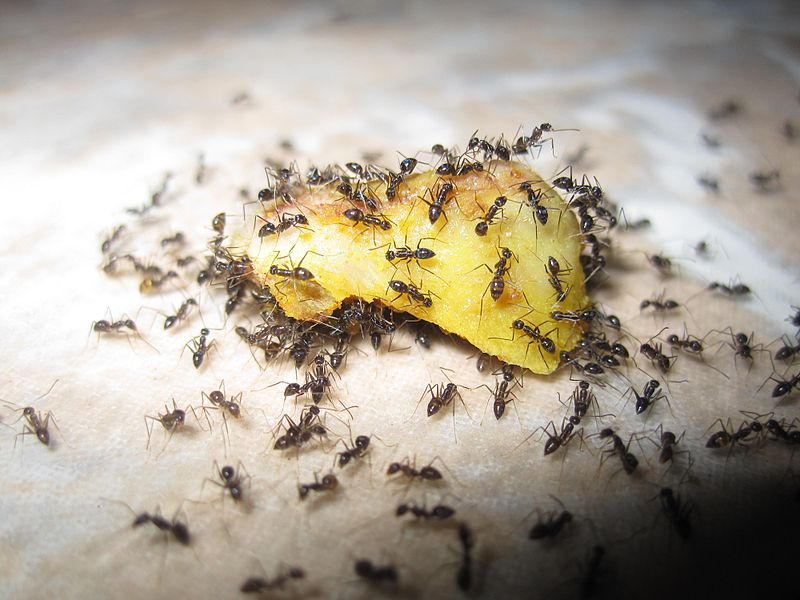
\includegraphics[width=4cm]{800px-Ants_eating_fruit}\vspace{1cm}}

\question{Why?}

\question{Computat{\redidot}onal Challenges\\
          \vspace{1cm}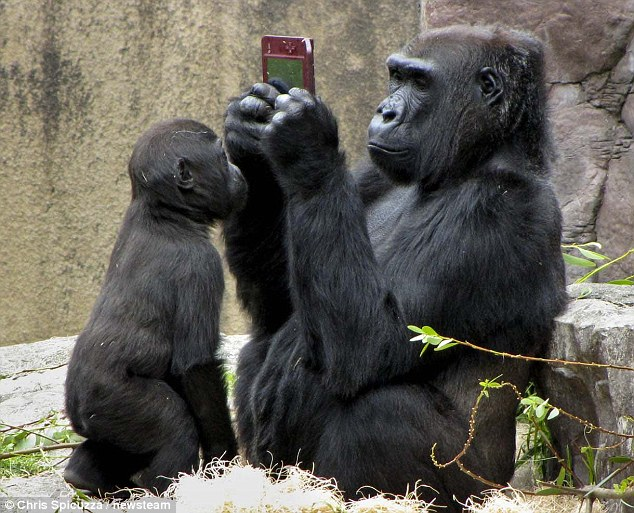
\includegraphics[width=4cm]{gorilla_tablet}}
\question{\red{Computat{\blackidot}onal} Challenges\\
          \vspace{1cm}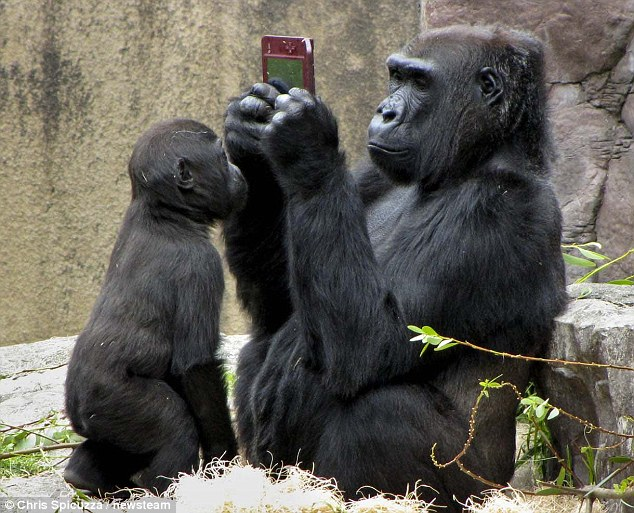
\includegraphics[width=4cm]{gorilla_tablet}}

\picw{Chinese-abacus}{}{1}{0}
\pic{book_and_screen}{}
\pic{8GB_vs_8Byte}{}

\frame{\frametitle{More and more diverse hardware}
 \abspic{05_intel_ivy_bridge}         {-0.20}{0.0}{0.4}
 \abspic{07_Nvidia_tesla_k10}         {-0.05}{0.4}{0.2}
 \abspic{10_KnightsCornerChip_in_hand}{ 0.10}{0.7}{0.25}
}
\picw{kraken}{}{1}{0}

\frame{\frametitle{Computational Challenges}
 \abspic{640px-Gorilla_Scratching_Head}{0.2}{0.5}{0.35}
 \begin{itemize}
 \item Simulate cutting edge science
 \item Use latest numerical methods
 \item Make use of latest hardware
  \begin{itemize}
  \item Cache
  \item Vector
  \item SMP parallelism
  \item GPU
  \item Scale to many nodes
  \end{itemize}
 \end{itemize}
}

\question{Collaborat{\redidot}ve Challenges\\
          \vspace{1cm}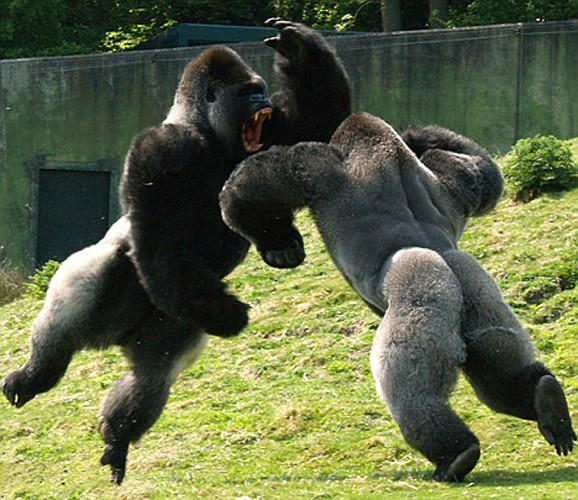
\includegraphics[width=4cm]{gorilla_fight}}
\question{\red{Collaborat{\blackidot}ve} Challenges\\
          \vspace{1cm}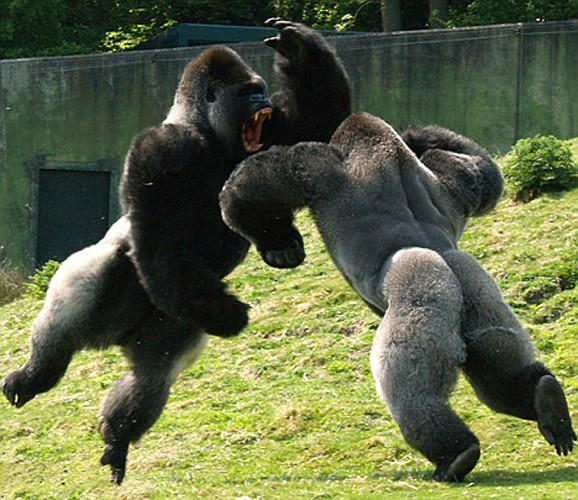
\includegraphics[width=4cm]{gorilla_fight}}

\frame{
  \abspic{community_only_problem}    {-0.1}{0.1}{0.6}
}

\frame{
  \abspic{community_with_problem}    {-0.1}{0.1}{0.6}
  \abspic{hurricane}     {-0.35}{0.05}{0.2}
  \abspic{wind_park}     {-0.30}{0.73}{0.2}
  \abspic{space_shuttle} { 0.20}{0.00}{0.2}
  \abspic{crab}          { 0.20}{0.75}{0.2}
}

\frame{
  \abspic{community_with_computation}{-0.1}{0.1}{0.6}
  \abspic{hurricane}     {-0.35}{0.05}{0.2}
  \abspic{wind_park}     {-0.30}{0.73}{0.2}
  \abspic{space_shuttle} { 0.20}{0.00}{0.2}
  \abspic{crab}          { 0.20}{0.75}{0.2}
  \abspic{kraken}        {-0.07}{0.40}{0.15}
  \abspic{tianhe1}       { 0.31}{0.40}{0.15}
}

\frame{
  \abspic{community_of_groups}       {-0.1}{0.1}{0.6}
  \abspic{hurricane}     {-0.35}{0.05}{0.2}
  \abspic{wind_park}     {-0.30}{0.73}{0.2}
  \abspic{space_shuttle} { 0.20}{0.00}{0.2}
  \abspic{crab}          { 0.20}{0.75}{0.2}
  \abspic{kraken}        {-0.07}{0.40}{0.15}
  \abspic{tianhe1}       { 0.31}{0.40}{0.15}
}

\frame{
  \abspic{community_of_groups}       {-0.1}{0.1}{0.6}
  \abspic{hurricane}     {-0.35}{0.05}{0.2}
  \abspic{wind_park}     {-0.30}{0.73}{0.2}
  \abspic{space_shuttle} { 0.20}{0.00}{0.2}
  \abspic{crab}          { 0.20}{0.75}{0.2}
  \abspic{email}         { 0.06}{0.38}{0.10}
  \abspic{phone}         { 0.04}{0.53}{0.10}
  \abspic{irc}           { 0.25}{0.40}{0.10}
  \abspic{www}           { 0.25}{0.55}{0.10}
}

\frame{
  \abspic{email}         { 0.06}{0.38}{0.10}
  \abspic{phone}         { 0.04}{0.53}{0.10}
  \abspic{irc}           { 0.25}{0.40}{0.10}
  \abspic{www}           { 0.25}{0.55}{0.10}
  \pause
  \abspic{Subversion-logo}{-0.28}{0.20}{0.23}
  \abspic{Git-logo}       {-0.20}{0.40}{0.13}
  \abspic{Mercurial_logo} {-0.20}{0.70}{0.13}
  \pause
  \abspic{Trac_logo}      { 0.10}{0.05}{0.10}
  \pause
  \abspic{Mediawiki_logo} { 0.10}{0.70}{0.15}
  \pause
  \abspic{Workshop}       { 0.35}{0.10}{0.05}
}

\frame{
  \abspic{community_with_problems}   {-0.1}{0.1}{0.6}
  \abspic{hurricane}     {-0.35}{0.05}{0.2}
  \abspic{wind_park}     {-0.30}{0.73}{0.2}
  \abspic{space_shuttle} { 0.20}{0.00}{0.2}
  \abspic{crab}          { 0.20}{0.75}{0.2}
}

\frame{
  \abspic{community_with_competition}{-0.1}{0.1}{0.6}
  \abspic{crab}          {-0.35}{0.05}{0.2}
  \abspic{crab}          {-0.30}{0.73}{0.2}
  \abspic{crab}          { 0.20}{0.00}{0.2}
  \abspic{crab}          { 0.20}{0.75}{0.2}
}

\frame{
  \abspic{community_with_standards}{-0.1}{0.1}{0.6}
  \abspic{hurricane}     {-0.35}{0.05}{0.2}
  \abspic{wind_park}     {-0.30}{0.73}{0.2}
  \abspic{space_shuttle} { 0.20}{0.00}{0.2}
  \abspic{crab}          { 0.20}{0.75}{0.2}
}

\frame{
  \abspic{community_with_standards}{-0.1}{0.1}{0.6}
  \abspic{hurricane}     {-0.35}{0.05}{0.2}
  \abspic{wind_park}     {-0.30}{0.73}{0.2}
  \abspic{space_shuttle} { 0.20}{0.00}{0.2}
  \abspic{crab}          { 0.20}{0.75}{0.2}
  \abspic{Imperial-Metric}{0.35}{0.40}{0.12}
  \pause
  \abspic{hdf_logo}      {-0.10}{0.45}{0.1}
}

\frame{
  \abspic{community_with_tools}{-0.1}{0.1}{0.6}
  \abspic{hurricane}     {-0.35}{0.05}{0.2}
  \abspic{wind_park}     {-0.30}{0.73}{0.2}
  \abspic{space_shuttle} { 0.20}{0.00}{0.2}
  \abspic{crab}          { 0.20}{0.75}{0.2}
}
\frame{
  \abspic{community_with_tools_examples}{-0.1}{0.1}{0.6}
}
\frame{
  \abspic{community_with_tools_examples}{-0.1}{0.1}{0.6}
  \abspic{Tux-linux_logo}     {-0.35}{0.05}{0.2}
  \abspic{Windows_logo}       {-0.30}{0.73}{0.2}
  \abspic{Apple_Logo}         { 0.20}{0.03}{0.15}
  \abspic{Tux-linux_logo}     { 0.17}{0.13}{0.2}
  \abspic{Apple_Logo}         { 0.24}{0.77}{0.15}
}

\frame{
  \abspic{community_with_credit}{-0.1}{0.1}{0.6}
  \abspic{hurricane}     {-0.35}{0.05}{0.2}
  \abspic{wind_park}     {-0.30}{0.73}{0.2}
  \abspic{space_shuttle} { 0.20}{0.00}{0.2}
  \abspic{crab}          { 0.20}{0.75}{0.2}
}
\frame{
  \abspic{community_with_credit}{-0.1}{0.1}{0.6}
  \abspic{crab}          {-0.35}{0.05}{0.2}
  \abspic{crab}          {-0.30}{0.73}{0.2}
  \abspic{crab}          { 0.20}{0.00}{0.2}
  \abspic{crab}          { 0.20}{0.75}{0.2}
}


\frame{\frametitle{Collaborative Challenges}
 \abspic{germany}              {-0.09}{0.36}{0.2}
 \abspic{germany_map}          { 0.12}{0.46}{0.2}
 \abspic{800px-Los_Angeles_Skyline_telephoto}{-0.05}{0.68}{0.2}
 \abspic{georgia}              { 0.26}{0.56}{0.18}
 \abspic{louisiana}            { 0.42}{0.37}{0.21}
 \abspic{neworleans}           { 0.45}{0.65}{0.18}
How can we work together?
\begin{itemize}
    \item Researchers in the USA
    \begin{itemize}
        \item Louisiana
        \item Pennsylvania
        \item Georgia
        \item California
    \end{itemize}
    \item Researchers in Germany
    \item Researchers in Canada
\end{itemize}
}

\frame{\frametitle{Einstein Toolkit as growing project}
 \abspic{jigsaw1} {-0.082}{0.35}{0.16}
 \vspace{-4cm}
 \begin{itemize}
  \item \small Initially: some infrastructure, some application code
 \end{itemize}
}
\frame{\frametitle{Einstein Toolkit as growing project}
 \abspic{jigsaw2} {-0.2}{0.2}{0.4}
 \vspace{-4cm}
 \begin{itemize}
  \item \small Growing application suite
 \end{itemize}
}
\frame{\frametitle{Einstein Toolkit as growing project}
 \abspic{jigsaw3} {-0.2}{0.14}{0.52}
 \vspace{-4cm}
 \begin{itemize}
  \item \small Growing infrastructure ``return''
 \end{itemize}
}
\frame{\frametitle{Einstein Toolkit as growing project}
 \abspic{jigsaw4} {-0.205}{0.135}{0.525}
 \vspace{-4cm}
 \begin{itemize}
  \item \small Users from more fields of science
 \end{itemize}
}
\frame{\frametitle{Einstein Toolkit as growing project}
 \abspic{jigsaw5} {-0.205}{0.135}{0.525}
 \vspace{-4cm}
 \begin{itemize}
  \item \small Most modules open-source, but not necessarily all
 \end{itemize}
}

\question{Base Modules\\*[1em]
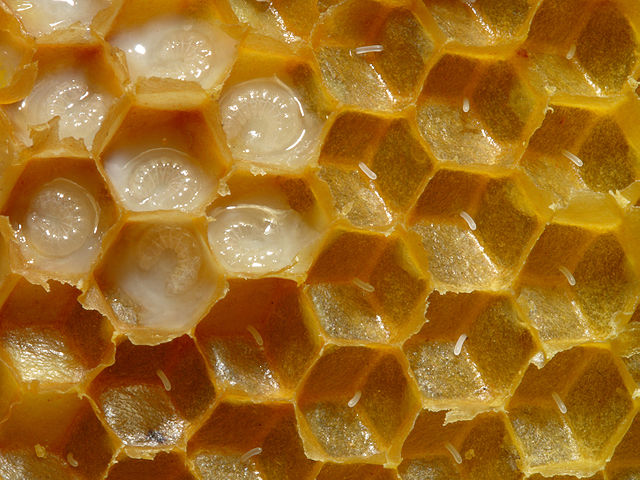
\includegraphics[width=0.4\textwidth]{640px-Bienenwabe_mit_Eiern_und_Brut_5}}

\frame{\frametitle{The Einstein Equations}
  \abspic{Eeq_Eeq}{-0.25}{0.0}{0.70}
}
\frame{
  \abspic{Eeq_curvature}{-0.25}{0.0}{0.70}
}
\frame{
  \abspic{Eeq_constants}{-0.25}{0.0}{0.70}
}
\frame{
  \abspic{Eeq_matter}{-0.25}{0.0}{0.70}
}
\frame{
  \abspic{Eeq_all}{-0.25}{0.0}{0.70}
}

\frame{
  \abspic{ET_layout_Eeq}{-0.25}{0.0}{0.70}
}
\frame{
  \abspic{ET_layout_ADMBase}{-0.25}{0.0}{0.70}
}
\frame{
  \abspic{ET_layout_Base2}{-0.25}{0.0}{0.70}
}
\frame{
  \abspic{ET_layout_Tmunu}{-0.25}{0.0}{0.70}
}
\frame{
  \abspic{ET_layout_inv_cowling}{-0.25}{0.0}{0.70}
}
\frame{
  \abspic{ET_layout_evolution}{-0.25}{0.0}{0.70}
}
\frame{
  \abspic{ET_layout_all}{-0.25}{0.0}{0.70}
}
\frame{
  \abspic{ET_layout_multiple}{-0.25}{0.0}{0.70}
}

\frame{\frametitle{Guiding Principles}
 \abspic{opensource_logo}{0.2}{0.7}{0.2}
 \begin{itemize}
  \item Open, community-driven software development
  \item Separation of \textbf{physics} software and \textbf{computational} infrastructure
  \item Stable interfaces, allowing extensions
  \item Simplify usage where possible:
   \begin{itemize}
    \item Doing science $>>$ Running a simulation
    \item Students need to know a lot about physics\\
           (meaningful initial conditions, numerical stability,\\
           accuracy/resolution, have patience, have curiosity,\\
           develop a ``gut feeling'' for what is right ...)
    \item Einstein Toolkit \textbf{cannot} give that, \textbf{however}:
    \item Open codes that are easy to use allow to concentrate on these things!
   \end{itemize}
 \end{itemize}
}

\frame{\frametitle{Credits, Citations}
 \abspic{barretr_Book.png}{0.2}{0.7}{0.2}
 In academics: citations, citations, citations!\\
 For Einstein Toolkit:
 \begin{itemize}
  \item Open and free source
  \item No \textbf{requirement} to cite anything
  \item However: \textbf{requested} to cite a few publications
  \item Which publications:
  \begin{itemize}
   \item One, maybe two for the Toolkit itself
   \item Some components list a few as well
   \item List published on website and manage through publication database
  \end{itemize}
 \end{itemize}
}

\section{Vision}
\frame{\frametitle{Vision}
 \abspic{arrow}{0}{0.65}{0.2}
 Near Future
 \begin{itemize}
  \item Inclusion of ``more physics'', e.g. general \\MHD, tabulated equations of state
  \item Improve scaling of existing mesh methods
 \end{itemize}
 Mid-term
 \begin{itemize}
  \item Neutrino radiation code
  \item Fundamental extension of numerical methods
  \item Requirement-base scheduling
 \end{itemize}
 Long-term
 \begin{itemize}
  \item Completely requirement-based programming
 \end{itemize}
}

\section{Summary}
\frame{\frametitle{Summary}
 \abspic{people}    {-0.15}{0.55}{0.15}
 \abspic{opensource_logo}{0.05}{0.8}{0.1}
 \begin{centering}
  \href{run:mplayer -noaspect -fs -zoom -vo xv ../pics/Einstein_Toolkit.avi}{
    
\includegraphics[height=2cm]{cactuslogo}}\\
 \end{centering}
 {\large Einstein Toolkit\\}
 \begin{itemize}
  \item http://einsteintoolkit.org/
  \item Tools for high-performance computing in numerical relativity
  \item Open Source
  \item World-wide, open Community
  \item Used in high-end research
 \end{itemize}
}

\end{document}

